Due to a change in the analysis procedure in the calculation of the Cs and laser
calibration constants, a reprocessing of the 2011 data was performed. Changing
the calibration constants, according to \cref{eq:70}, changes the reconstructed
energy in the cell thus affecting the jet identification (see
\cref{sec:topocluster}). A comparison between the $phi$--averaged RMS of
electronic cell noise as a function of $\eta$ of the cell before and after
reprocessing for the high statistic 192130 run with both channels in high gain
is shown in \cref{fig:noise_avg_old_new_hghg}. There is a general increase of
the cell noise in the EBC, LBC and EBA partitions, the LBA partition had module
22 running in \emph{emergency mode}, i.e.\ operated with $\sim$ 50~V less high
voltage on the PMTs, and had the cesium calibration constants updated this
change lowered the average noise in this partition.

\begin{figure}[!h]
  \centering
    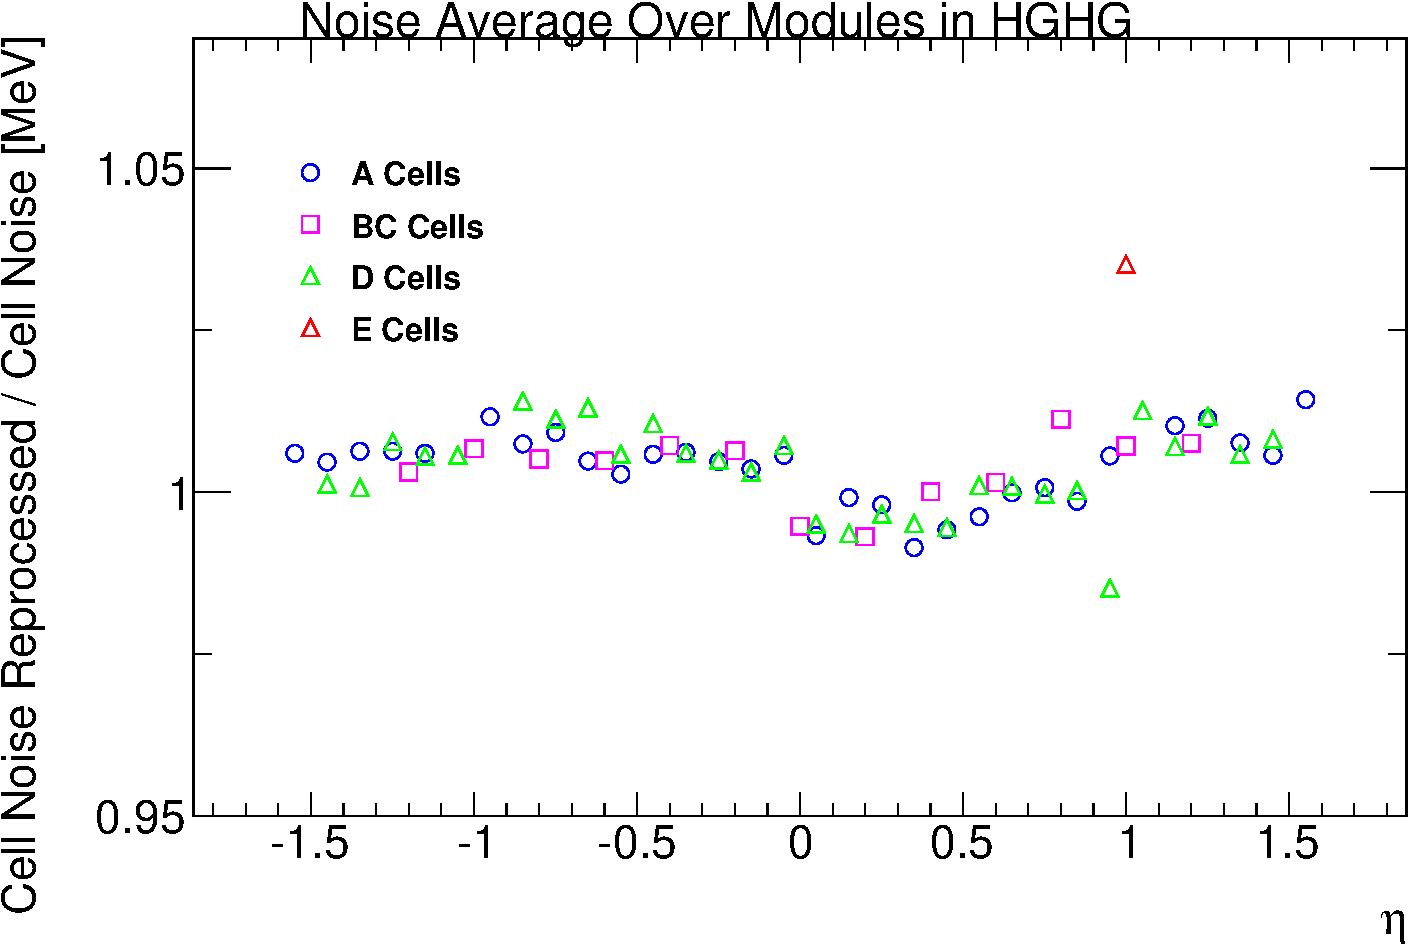
\includegraphics[width=.7\linewidth]{noise_avg_old_new_192130_hghg}
    \caption{Comparison between the $phi$--averaged RMS of electronic cell noise
      as a function of $\eta$ of the cell before and after reprocessing for the
      high statistic 192130 run with both channels in high gain. The different
      layers are shown separately, A, BC, D and E (gap/crack). The transition
      between the long and extended barrels can be seen in the range
      $0.7 < |\eta| < 1.0$.}
    \label{fig:noise_avg_old_new_hghg}
\end{figure}

The change of the cell noise between IOVs was monitored using a special software
within the TUCS environment. A problem with the TNF was spotted where a
variation in the cell noise without a corresponding variation in other relevant
quantities were present. The number of cells affected by this problem is
investigated constructing the distribution of the ratio $\sigma$ /
RMS$_\mathrm{\, eff}$ (see \cref{fig:all_rms_eff}). This distribution is assumed
to be Gaussian around 1 in order to calculate the standard deviation
($\sigma_0$). The number of cells with a ratio $\sigma$ / RMS$_\mathrm{\, eff}$
$> 1 + 3 \sigma_0$ is 276 which corresponds approximately to the 5\% of the
detector.

After the installation of the new LVPS the electronic noise can be described
with a single Gaussian model thus the TNF is expected to have less impact and no
further studies have been made.

\begin{figure}[!h]
  \centering
    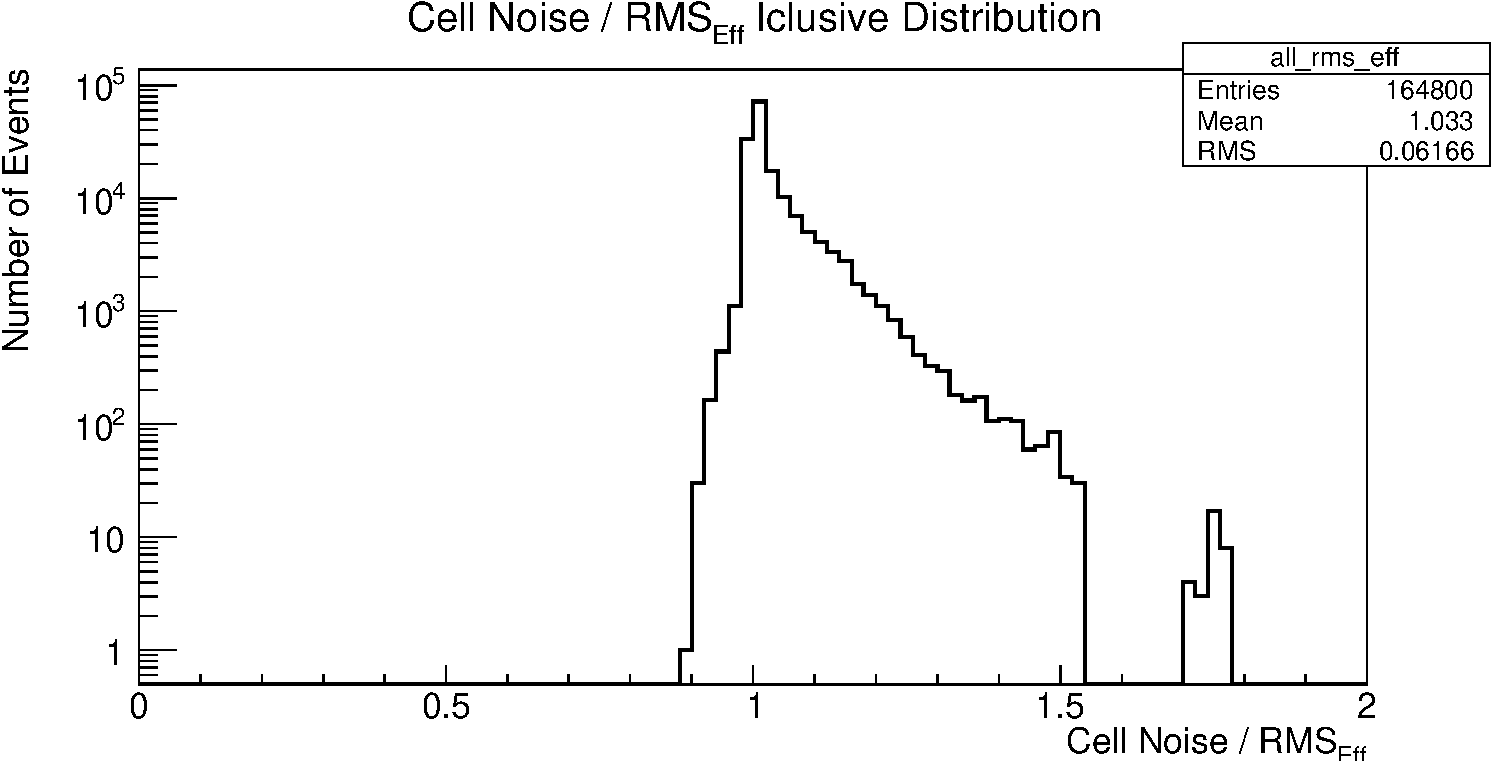
\includegraphics[width=.7\linewidth]{all_rms_eff}
    \caption{Histogram of the ratio $\sigma$ / RMS$_\mathrm{\, eff}$ where the
      $\sigma$ and RMS$_\mathrm{\, eff}$ values are taken from all IOVs in 2011.}
    \label{fig:all_rms_eff}
\end{figure}
%%% Local Variables:
%%% mode: latex
%%% TeX-master: "../search_for_DM_LED_with_ATLAS"
%%% End:
